\tightsection{How Predictable Are Video Metrics?}
\label{predictability}

\comment{
<<<<<<< HEAD
\jc{Make sure to use ``session'' and ``quality sample'' consistently, and ``quality'' and ``performance'' consistently}

The quality of a video session depends on a variety of factors,
including the network and the CDN. While many of these factors are not
under our control, some of them are. In our case, we assume that we
can control the bitrate of the session, as well as the CDN it streams
from. The challenge is that we do not know what quality will a session
exhibit given a particular choice of the parameters we can
control. This means that making any decision to change the CDN or the
bitrate is more or less like ``shooting in the dark''.

To address this problem, we start with the assumption that the session
quality is correlated to different characteristics (attributes)
associated with the session. Example of such attributes are CDN,
bitrate, ISP, IP address, device, connectivity type, etc. We say that
a session is {\it predictable} if given the values of the attributes
associated with the session we can predict its quality. 

In this section, we formally define {\it predictability}, as well as
provide an upper bound to help us evaluate different prediction
algorithms (\Section~\ref{subsec:upperbound}). We then use our data
set to quantify this upper bound
(\Section~\ref{subsec:videoupperbound}).
}
%The quality outcome of a session which we would like to predict (which we will call the {\it session under prediction}) intuitively result from a diverse set of factors -- user behavior, network behavior, and CDN behavior, to name a few.  Many of these factors are out of our control; in other cases, a factor may be impacted in principle but its dependence on our decisions is unpredictable.  Our hope in approaching this problem is that some of them, and their causal dependence on decisions we can take, are consistently associated with characteristics we observe about sessions.  As shorthand we say that quality is {\it predictable} to extent that the impact of available decisions can be predicted, with low average error, using the available information about attributes of a session.  The first empirical question we must answer is whether quality is predictable in our dataset. 

%In this section, we first introduce the {\it predictability} and its upper bound of a set of sessions against a simple abstract model of prediction algorithm (\Section~\ref{subsec:upperbound}). Note that since the predictability is defined against a class of prediction algorithms that we consider rather than one specific design, its upper bound provides the insight of the intrinsic difficulty in predicting a set of sessions. We also quantify the predictability upper bound of video quality using our dataset (\Section~\ref{subsec:videoupperbound}). 


%=======
Before we delve into algorithms, we are first going to answer the question of how ``preditable'' are the video metrics using the client-side session-level attributes. Intuitively, if all sessions with the same attribute values exhibit same or similar video quality, then the set of attributes are predictive of video quality metrics, and vice versa. In this section, we will present an empirical predictability analysis based on real-world data. Such analysis also establishes a lower bound of the prediction error that can help us evaluate the prediction algorithm presented in \Section~\ref{sec:prediction}.
%>>>>>>> a13c3cc981c87551f3a5c5447b0cd17e6b3937fd

\tightsubsection{Definitions}
\label{subsec:definitions}

%We first define predictability. 


\myparatight{Prediction error} We start with defining the {\it prediction error}.  Given a session
(which we will call the {\it session under prediction}), let $q$ be
the actual quality and $p$ be the predicted quality\footnote{We consider one quality metric at a time.}. Then, the
prediction error $e_{p,q}=|p-q|$.
For a set of session under prediction $S=\{s_1,\dots,s_n\}$, let $P=\{p_i\}$ and $Q=\{q_i\}$ be their predicted and actual qualities. respectively ($p_i$ and $q_i$ are the predicted and actual quality of $s_i$). The overall prediction error is then the square root of mean squre error of $P$ and $Q$, $E_{P,Q}=\left(\frac{1}{n}\sum e_{p_i,q_i}^2\right)^{1/2}$.

\myparatight{Attribute combination (AC)} The informatino associated to a session under prediction includes the values of multiple attributes (see \Section~\ref{subsec:dataset}). We define {\it attribute combination} ({\it AC}) $g$ to be a set of attributes, e.g. $[ASN, CDN]$. Then the attribute combination value of session $s$ on AC $g$, denoted as $v_g(s)$, is a tuple of values on all attributes in $g$ associated to $s$. For example, if $g=[ASN,CDN]$ and $s$ is a session from a host in $ASN1$ to $CDN1$, $v_g(s)=[ASN1, CDN1]$. We say two sessions are identical with respect to an AC, if they produce the same attribute combination values. Using such equivalence relationship, an AC $g$ can be used to partition a set of sessions into groups (called, {\it identical groups}) such that two sessions in an identical group are identical with respect to $g$.
In addition to the attributes in \Section~\ref{subsec:dataset}, we also consider temporal attributes. For instance, given AC $g=[ASN, CDN, 5\,minute]$, two sessions are identical only if they belong to the same ASN, use the same CDN and they are received within the same 5-minute interval. The temporal attributes are useful according to previous research~\cite{sigcomm12} which shows temporal variability of video quality within the same class of sessions.
\xil{I think this can be further cleaner.}


% xil: I feel like this is a simple concept that can be captured with plain English.
%We define {\it attribute combination} ({\it AC}) $g$ to be a set of attributes. Given an AC $g$, function $v_g$ takes a session $s$ as input and returns an array of values of $s$ on each attribute in $g$. For instance, if $g=[\textrm{ASN, CDN}]$, $v_g(s)=[ASN_s,CDN_s]$ where the client of $s$ belongs to $ASN_s$ and the server belongs to $CDN_s$. An {\it attribute-based prediction algorithm} $P$ \ion{$P$ is also the predicted quality vector, so need to change the notation.} is defined by an AC $g$. $P$ takes a session $s$ as input, and returns $P_g(s)$ as the predicted quality. Note that such an algorithm will provide the same prediction to all sessions with identical attribute values. This means that $P$ cannot provide perfect prediction unless we identify all possible attributes that may impact a sessions's quality, which in practice is infeasible.

%We define {\it attribute combination} ({\it AC}) $g$ to be a set of attributes, e.g. $[ASN, CDN]$. An AC is used to partition a set of quality samples. In addition, we also consider temporal attributes, for example, ...



%\xil{the point of the next sentence is unclear.} Note that such an algorithm will provide the same prediction to all sessions with identical attribute values. This means that $P$ cannot provide perfect prediction unless we identify all possible attributes that may impact a sessions's quality, which in practice is infeasible.

\myparatight{Attribute-based prediction algorithm}
An {\it attribute-based prediction algorithm} takes a session $s$ (with no quality information) and an AC $g$ as input, and returns the predicted quality of $s$. This means that if a set of sessions are received when the algorithm is given the same AC, their predicted qualities only depend on their values on $g$. Specifically, if they are identical with respect to $g$, they should be given the same predicted quality.\jc{some justification to support this assumption is needed.} 
\xil{hard to read}\jc{Fixed?}

\tightsubsection{Lower bound of prediction error}
\label{subsec:lowerbound}
This assumption naturally leads to an {\it lower bound} of prediction error of any algorithm in this kind. 
The idea is that given an AC $g$ and an identical group of sessions $S=\{s_1,\dots,s_n\}$, the overall prediction error $\left(\frac{1}{n}\sum e_{p,q_i}^2\right)^{1/2}$ is minimized when the prediction $p$ for each of them is the mean of $q_i$. Furthermore, if $S$ is partitioned into multiple identical groups,  the overall prediction error is minimized when the prediction for each group is the mean of actual quality of these sessions in the group. 
\xil{maybe add a pointer to basic statistics?}\jc{didn't find any}

%The {\it predictability} of a particular AC over a set of sessions is the minimal overall prediction error that can be achieved, i.e., $\textrm{argmax}E_{P,Q}=\textrm{argmax}_p\left(\frac{1}{n}\sum e_{p,q_i}^2\right)^{1/2}$


%For example, the optimal buffering ratio prediction for a session from a group is to predict using the mean of buffering ratio from that group. 
Intuitively, this lower bound characterizes the dispersion in quality of the sessions which an AC cannot differentiate. Ideally, if the attributes selected in AC reflect all the factors that determine the quality of a session, the sessions in an identical group should produce the same quality and the lower bound is zero. However, given the limitation of measurement and nature of noises (see \Section~\ref{sec:challenges} for detailed discussion), it is expected that such lower bound is non-trivial and should to be quantified empiracally.


%Therefore, the predicability of $g$ over a session set $S$ is the minimal overall prediction error $R_g(S)=E_{P^*,Q}$ where $P^*$ gives the same optimal prediction $p^*$ for each session in $S$. This definition can be extended to any set of sessions $S$ by dividing sessions into identical groups of $g$, and use the optimal prediction for each identical group to be the prediction of sessions in it, i.e., $R_g(S)=E_{P^*,Q}$ where prediction of $s_i$ in $P^*$ is the optimal prediction of the identical group that $s_i$ belongs to.\ion{This is a very confusing paragraph.}


%The {\it predictability} of AC $g$ over a set of sessions $S$ is the minimal overal prediction error over all prediction algorithms on $g$, i.e., $p^*=\textrm{argmax}E_{P,Q}=\textrm{argmax}_p\left(\frac{1}{n}\sum e_{p,q_i}^2\right)^{1/2}$. For example, the optimal buffering ratio prediction for a session from a group is to predict using the mean of buffering ratio from that group. Therefore, the predicability of $g$ over a session set $S$ is the minimal overall prediction error $R_g(S)=E_{P^*,Q}$ where $P^*$ gives the same optimal prediction $p^*$ for each session in $S$. This definition can be extended to any set of sessions $S$ by dividing sessions into identical groups of $g$, and use the optimal prediction for each identical group to be the prediction of sessions in it, i.e., $R_g(S)=E_{P^*,Q}$ where prediction of $s_i$ in $P^*$ is the optimal prediction of the identical group that $s_i$ belongs to.\ion{This is a very confusing paragraph.} 

%The predictability quantifies the dispersion in quality of the sessions that an AC cannot differentiate. Ideally, if the attributes in AC $g$ selected reflect all the factors that determine the quality of a session, then the sessions in an identical group of $g$ should produce the same quality and the upper bound is exactly one. 

%\jc{The current definition predictability is weird as it gives smaller value to more predictable set of sessions. }


\begin{figure}[h!]
\centering
\subfigure[Temporal attributes]
{
	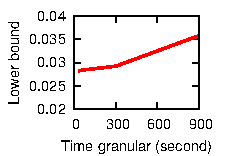
\includegraphics[width=0.24\textwidth]{figures/newfig/lowerbound-temp-metricId0.pdf}
	\label{subfig:predictability:temporal}
}
\hspace{-0.6cm}
\subfigure[Spatial attributes]
{
	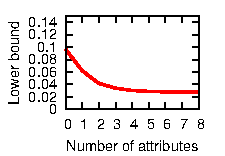
\includegraphics[width=0.24\textwidth]{figures/newfig/lowerbound-spatial-temp1-metricId0.pdf}
	\label{subfig:predictability:spatial}
}
\hspace{-0.6cm}
\subfigure[Per-ASN]
{
	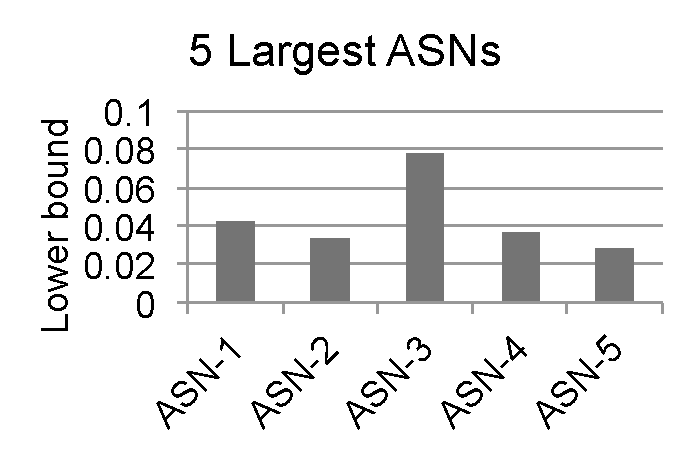
\includegraphics[width=0.24\textwidth]{figures/newfig/bar-predictability-asn.pdf}
	\label{subfig:predictability:asn}
}
\hspace{-0.6cm}
\subfigure[Per-Site]
{
	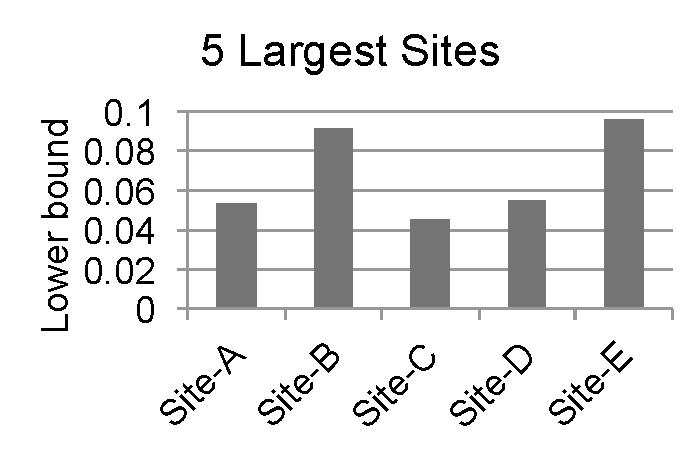
\includegraphics[width=0.24\textwidth]{figures/newfig/bar-predictability-site.pdf}
	\label{subfig:predictability:site}
}
\tightcaption{Empirical analysis for lower bound. Quantifying impact of different factors on the lower bound of prediction error of buffering ratio over our dataset.}
\label{fig:predictability}
\end{figure}


\tightsubsection{Empirical lower bound analysis}

%\xil{need some clean up after figures are in, describe data set, set up ``time is an attribute" (maybe even before)}

In this section, we quantify the prediction error lower bound (we use lower bound for short) of the attributes in our dataset. Note that such lower bound is not necessarily tight as it uses the information of the actual qualities of sessions under prediction. Moreover, it does not bound the performance of algorithms that are not attribute-based (e.g., video quality can be affected by factors that are not characterized by our attributes).
Despite these limitations, predictability is a valuable bound to compare prediction algorithms agianst. We consider the set of spatial attributes introduced in \Section~\ref{subsec:dataset} as well as a set of time intervals as temporal attributes.

\myparatight{Temporal attributes} Figure~\ref{subfig:predictability:temporal} shows the lower bound of different temporal attributes (time granular) combined with all spatial attributes. The value corresponding to $t-$second in the figure represents the lower bound of using t-seconds as temporal attribute, together with all spatial attributes introduced in \Section~\ref{subsec:dataset}. The lower bound tends to be better for small intervals. As the interval length increases the predictability stabilizes. 

\myparatight{Spatial attributes} In Figure~\ref{subfig:predictability:spatial}, we fix the temporal attribute to 1-minute and show the lower bound of different spatial attributes. Again, the finest spatial attribute combination is [ASN, Object, Site, Initial CDN, Initial Bitrate, OS, ConnectionType].  Instead of showing all ACs with these attributes (in total $2^7-1=127$ ACs), we group them by their number of attributes and show the ones with lowest lower bound. This illustrates the impact of the number of attributes on the lower bound. The results show clear improvements as we use more attributes, though we reach diminishing return when we approach seven attributes.

\myparatight{Different partitions} The above results show that the lower bound varies significantly with the attributes we consider. Next, we present the lower bound also varies across different partitions of the same AC (e.g., ASN, Site). Figure~\ref{subfig:predictability:asn} and~\ref{subfig:predictability:site} show the mean of lower bound of prediction in buffering ratio for the most largest 5 ASNs and Sites. These results confirm that the lower bound vary significantly across different spatial partitions, i.e., the attributes are more predictive in certain cases than others. %As shown in the next section, this mostly likely indicates there are attributes we do not collect that affect performance in certain scenarios. \xil{make sure last sentence is correct.}

In summary, we showed that in general, the session attributes we chose are quite predictive of video quality metrics, with a lower bound prediction error of less than 3\%.


